% Options for packages loaded elsewhere
\PassOptionsToPackage{unicode}{hyperref}
\PassOptionsToPackage{hyphens}{url}
\PassOptionsToPackage{dvipsnames,svgnames,x11names}{xcolor}
%
\documentclass[
  12pt,
  openany]{book}
\title{Systematic Microbiome Data Analysis in R}
\usepackage{etoolbox}
\makeatletter
\providecommand{\subtitle}[1]{% add subtitle to \maketitle
  \apptocmd{\@title}{\par {\large #1 \par}}{}{}
}
\makeatother
\subtitle{End to End Practical User Guides}
\author{Teresia Mrema-Buza, A Microbiome Data Science Enthusiast and Owner of the Complex Data Insights, LLC, USA}
\date{2022-05-21}

\usepackage{amsmath,amssymb}
\usepackage{lmodern}
\usepackage{iftex}
\ifPDFTeX
  \usepackage[T1]{fontenc}
  \usepackage[utf8]{inputenc}
  \usepackage{textcomp} % provide euro and other symbols
\else % if luatex or xetex
  \usepackage{unicode-math}
  \defaultfontfeatures{Scale=MatchLowercase}
  \defaultfontfeatures[\rmfamily]{Ligatures=TeX,Scale=1}
  \setmainfont[]{Times New Roman}
\fi
% Use upquote if available, for straight quotes in verbatim environments
\IfFileExists{upquote.sty}{\usepackage{upquote}}{}
\IfFileExists{microtype.sty}{% use microtype if available
  \usepackage[]{microtype}
  \UseMicrotypeSet[protrusion]{basicmath} % disable protrusion for tt fonts
}{}
\makeatletter
\@ifundefined{KOMAClassName}{% if non-KOMA class
  \IfFileExists{parskip.sty}{%
    \usepackage{parskip}
  }{% else
    \setlength{\parindent}{0pt}
    \setlength{\parskip}{6pt plus 2pt minus 1pt}}
}{% if KOMA class
  \KOMAoptions{parskip=half}}
\makeatother
\usepackage{xcolor}
\IfFileExists{xurl.sty}{\usepackage{xurl}}{} % add URL line breaks if available
\IfFileExists{bookmark.sty}{\usepackage{bookmark}}{\usepackage{hyperref}}
\hypersetup{
  pdftitle={Systematic Microbiome Data Analysis in R},
  pdfauthor={Teresia Mrema-Buza, A Microbiome Data Science Enthusiast and Owner of the Complex Data Insights, LLC, USA},
  colorlinks=true,
  linkcolor={Maroon},
  filecolor={Maroon},
  citecolor={Blue},
  urlcolor={Blue},
  pdfcreator={LaTeX via pandoc}}
\urlstyle{same} % disable monospaced font for URLs
\usepackage[margin=1in]{geometry}
\usepackage{color}
\usepackage{fancyvrb}
\newcommand{\VerbBar}{|}
\newcommand{\VERB}{\Verb[commandchars=\\\{\}]}
\DefineVerbatimEnvironment{Highlighting}{Verbatim}{commandchars=\\\{\}}
% Add ',fontsize=\small' for more characters per line
\usepackage{framed}
\definecolor{shadecolor}{RGB}{248,248,248}
\newenvironment{Shaded}{\begin{snugshade}}{\end{snugshade}}
\newcommand{\AlertTok}[1]{\textcolor[rgb]{0.94,0.16,0.16}{#1}}
\newcommand{\AnnotationTok}[1]{\textcolor[rgb]{0.56,0.35,0.01}{\textbf{\textit{#1}}}}
\newcommand{\AttributeTok}[1]{\textcolor[rgb]{0.77,0.63,0.00}{#1}}
\newcommand{\BaseNTok}[1]{\textcolor[rgb]{0.00,0.00,0.81}{#1}}
\newcommand{\BuiltInTok}[1]{#1}
\newcommand{\CharTok}[1]{\textcolor[rgb]{0.31,0.60,0.02}{#1}}
\newcommand{\CommentTok}[1]{\textcolor[rgb]{0.56,0.35,0.01}{\textit{#1}}}
\newcommand{\CommentVarTok}[1]{\textcolor[rgb]{0.56,0.35,0.01}{\textbf{\textit{#1}}}}
\newcommand{\ConstantTok}[1]{\textcolor[rgb]{0.00,0.00,0.00}{#1}}
\newcommand{\ControlFlowTok}[1]{\textcolor[rgb]{0.13,0.29,0.53}{\textbf{#1}}}
\newcommand{\DataTypeTok}[1]{\textcolor[rgb]{0.13,0.29,0.53}{#1}}
\newcommand{\DecValTok}[1]{\textcolor[rgb]{0.00,0.00,0.81}{#1}}
\newcommand{\DocumentationTok}[1]{\textcolor[rgb]{0.56,0.35,0.01}{\textbf{\textit{#1}}}}
\newcommand{\ErrorTok}[1]{\textcolor[rgb]{0.64,0.00,0.00}{\textbf{#1}}}
\newcommand{\ExtensionTok}[1]{#1}
\newcommand{\FloatTok}[1]{\textcolor[rgb]{0.00,0.00,0.81}{#1}}
\newcommand{\FunctionTok}[1]{\textcolor[rgb]{0.00,0.00,0.00}{#1}}
\newcommand{\ImportTok}[1]{#1}
\newcommand{\InformationTok}[1]{\textcolor[rgb]{0.56,0.35,0.01}{\textbf{\textit{#1}}}}
\newcommand{\KeywordTok}[1]{\textcolor[rgb]{0.13,0.29,0.53}{\textbf{#1}}}
\newcommand{\NormalTok}[1]{#1}
\newcommand{\OperatorTok}[1]{\textcolor[rgb]{0.81,0.36,0.00}{\textbf{#1}}}
\newcommand{\OtherTok}[1]{\textcolor[rgb]{0.56,0.35,0.01}{#1}}
\newcommand{\PreprocessorTok}[1]{\textcolor[rgb]{0.56,0.35,0.01}{\textit{#1}}}
\newcommand{\RegionMarkerTok}[1]{#1}
\newcommand{\SpecialCharTok}[1]{\textcolor[rgb]{0.00,0.00,0.00}{#1}}
\newcommand{\SpecialStringTok}[1]{\textcolor[rgb]{0.31,0.60,0.02}{#1}}
\newcommand{\StringTok}[1]{\textcolor[rgb]{0.31,0.60,0.02}{#1}}
\newcommand{\VariableTok}[1]{\textcolor[rgb]{0.00,0.00,0.00}{#1}}
\newcommand{\VerbatimStringTok}[1]{\textcolor[rgb]{0.31,0.60,0.02}{#1}}
\newcommand{\WarningTok}[1]{\textcolor[rgb]{0.56,0.35,0.01}{\textbf{\textit{#1}}}}
\usepackage{longtable,booktabs,array}
\usepackage{calc} % for calculating minipage widths
% Correct order of tables after \paragraph or \subparagraph
\usepackage{etoolbox}
\makeatletter
\patchcmd\longtable{\par}{\if@noskipsec\mbox{}\fi\par}{}{}
\makeatother
% Allow footnotes in longtable head/foot
\IfFileExists{footnotehyper.sty}{\usepackage{footnotehyper}}{\usepackage{footnote}}
\makesavenoteenv{longtable}
\usepackage{graphicx}
\makeatletter
\def\maxwidth{\ifdim\Gin@nat@width>\linewidth\linewidth\else\Gin@nat@width\fi}
\def\maxheight{\ifdim\Gin@nat@height>\textheight\textheight\else\Gin@nat@height\fi}
\makeatother
% Scale images if necessary, so that they will not overflow the page
% margins by default, and it is still possible to overwrite the defaults
% using explicit options in \includegraphics[width, height, ...]{}
\setkeys{Gin}{width=\maxwidth,height=\maxheight,keepaspectratio}
% Set default figure placement to htbp
\makeatletter
\def\fps@figure{htbp}
\makeatother
\setlength{\emergencystretch}{3em} % prevent overfull lines
\providecommand{\tightlist}{%
  \setlength{\itemsep}{0pt}\setlength{\parskip}{0pt}}
\setcounter{secnumdepth}{5}
\usepackage{booktabs}
\usepackage{amsthm}
\makeatletter
\def\thm@space@setup{%
  \thm@preskip=8pt plus 2pt minus 4pt
  \thm@postskip=\thm@preskip
}
\makeatother
\usepackage{setspace}
\newpage
\newenvironment{tmbinfo}[0]{}{}
\renewenvironment{tmbinfo}[0]{}{}
\newenvironment{tmbalert}[0]{}{}
\renewenvironment{tmbalert}[0]{}{}
\newenvironment{tmbshare}[0]{}{}
\renewenvironment{tmbshare}[0]{}{}
\ifLuaTeX
  \usepackage{selnolig}  % disable illegal ligatures
\fi
\usepackage[]{natbib}
\bibliographystyle{apalike}

\begin{document}
\maketitle

{
\hypersetup{linkcolor=}
\setcounter{tocdepth}{1}
\tableofcontents
}
\hypertarget{frontpage}{%
\chapter*{Bioinformatics Analysis of Microbiome Data}\label{frontpage}}
\addcontentsline{toc}{chapter}{Bioinformatics Analysis of Microbiome Data}

Quick Glimpse

Microbiome data analysis is about asking questions to understand the microbial composition in a given sample. The Systematic Microbiome Data Analytics (\textbf{SMDA}) book series represent practical guides supporting the microbiome data analytics beyond the traditional analysis. This on-going project supports the transformation of complex microbiome data into optimal biological insights. For simplicity, the eBook is divided in four parts (Part 21 through Part 4). These series provide users with integrated solutions for gaining insight into microbial community biodiversity and investigating their role in disease, health and their impact in the environment.

License


\includegraphics[width=1.04167in,height=\textheight]{images/CCbyNCND.png} The online version of this book is free and licensed under a Creative Commons Attribution-NonCommercial-NoDerivatives 4.0 International License. The code that built this guide is available at a private GitHub repository. A minimal code and quick description of the book is available at a public \href{https://tmbuza.github.io/Systematic-Microbiome-Data-Analysis/}{GitHub Page}. If interested you can obtain a more detailed copy from the \href{https://complexdatainsights.com/products}{CDI LLC Store}.

\hypertarget{part-bioinformatics-analysis}{%
\part{BIOINFORMATICS ANALYSIS}\label{part-bioinformatics-analysis}}

\hypertarget{preprocessing-16S-reads}{%
\chapter{Preprocessing 16S rRNA Sequencing Data}\label{preprocessing-16S-reads}}

\hypertarget{initial-read-quality-scores}{%
\section{Initial read quality scores}\label{initial-read-quality-scores}}

We will use fastqc software to explore the original read qualities before trimming and decontamination.

\begin{Shaded}
\begin{Highlighting}[]
\FunctionTok{mkdir}\NormalTok{ data/fastqc1}
\ExtensionTok{fastqc} \PreprocessorTok{*}\NormalTok{.fastq.gz }\AttributeTok{{-}o}\NormalTok{ data/fastqc1}
\end{Highlighting}
\end{Shaded}

\begin{Shaded}
\begin{Highlighting}[]
\FunctionTok{mkdir}\NormalTok{ data/multiqc1}
\ExtensionTok{multiqc} \AttributeTok{{-}f} \AttributeTok{{-}{-}data{-}dir}\NormalTok{ data/fastqc1 }\AttributeTok{{-}o}\NormalTok{ data/multiqc1 }\AttributeTok{{-}{-}export}
\end{Highlighting}
\end{Shaded}

\begin{quote}
Plots from \texttt{multiqc} are exported to \texttt{multiqc\_plots} folder.
\end{quote}

\begin{figure}
\centering
\includegraphics[width=1\textwidth,height=\textheight]{data/multiqc1/multiqc_plots/png/mqc_fastqc_per_base_sequence_quality_plot_1.png}
\caption{Original: Mean quality scores}
\end{figure}

\begin{figure}
\centering
\includegraphics[width=1\textwidth,height=\textheight]{data/multiqc1/multiqc_plots/png/mqc_fastqc_per_sequence_quality_scores_plot_1.png}
\caption{Original: Per sequence quality scores}
\end{figure}

\hypertarget{read-trimming-using-bbduk.sh-from-bbmap-platform}{%
\section{\texorpdfstring{Read trimming using \texttt{bbduk.sh} from bbmap platform}{Read trimming using bbduk.sh from bbmap platform}}\label{read-trimming-using-bbduk.sh-from-bbmap-platform}}

\begin{quote}
Hint! Make sure that the pattern in the script is in the file name. Some files may contain \texttt{R1\_001.fastq.gz}. Here we use files downloaded from NCBI-SRA, they do not use R1\_001 in the sample name.
\end{quote}

\begin{Shaded}
\begin{Highlighting}[]
\ControlFlowTok{for}\NormalTok{ i }\KeywordTok{in} \KeywordTok{\textasciigrave{}}\FunctionTok{ls} \AttributeTok{{-}1} \PreprocessorTok{*}\NormalTok{\_1.fastq.gz }\KeywordTok{|} \FunctionTok{sed} \StringTok{\textquotesingle{}s/\_1.fastq.gz//\textquotesingle{}}\KeywordTok{\textasciigrave{}}
  \ControlFlowTok{do}
  \ExtensionTok{bbduk.sh} \AttributeTok{{-}Xmx4g}\NormalTok{ in1=}\VariableTok{$i}\DataTypeTok{\textbackslash{}\_}\NormalTok{1.fastq.gz in2=}\VariableTok{$i}\DataTypeTok{\textbackslash{}\_}\NormalTok{2.fastq.gz out1=data/trimmed/}\VariableTok{$i}\DataTypeTok{\textbackslash{}\_}\NormalTok{1.fastq.gz out2=data/trimmed/}\VariableTok{$i}\DataTypeTok{\textbackslash{}\_}\NormalTok{2.fastq.gz qtrim=r trimq=25 overwrite=True}
  \ControlFlowTok{done}
\end{Highlighting}
\end{Shaded}

\begin{Shaded}
\begin{Highlighting}[]
\FunctionTok{mkdir} \AttributeTok{{-}p}\NormalTok{ data/stats2  }
\ExtensionTok{seqkit}\NormalTok{ stat data/trimmed/}\PreprocessorTok{*}\NormalTok{.fastq.gz }\OperatorTok{\textgreater{}}\NormalTok{data/stats2/seqkit\_stats.txt}

\FunctionTok{mkdir}\NormalTok{ data/fastqc2}
\ExtensionTok{fastqc}\NormalTok{ data/trimmed/}\PreprocessorTok{*}\NormalTok{.fastq.gz }\AttributeTok{{-}o}\NormalTok{ data/fastqc2}

\FunctionTok{mkdir}\NormalTok{ data/multiqc2}
\ExtensionTok{multiqc} \AttributeTok{{-}f} \AttributeTok{{-}{-}data{-}dir}\NormalTok{ data/fastqc2 }\AttributeTok{{-}o}\NormalTok{ data/multiqc2 }\AttributeTok{{-}{-}export}
\end{Highlighting}
\end{Shaded}

\begin{figure}
\centering
\includegraphics[width=1\textwidth,height=\textheight]{data/multiqc2/multiqc_plots/png/mqc_fastqc_per_base_sequence_quality_plot_1.png}
\caption{Trimmed: Mean quality scores}
\end{figure}

\begin{figure}
\centering
\includegraphics[width=1\textwidth,height=\textheight]{data/multiqc2/multiqc_plots/png/mqc_fastqc_per_sequence_quality_scores_plot_1.png}
\caption{Trimmed: Per sequence quality scores}
\end{figure}

\hypertarget{read-decontamination}{%
\section{Read decontamination}\label{read-decontamination}}

\begin{itemize}
\tightlist
\item
  Using \texttt{bbduk.sh} from bbmap platform
\item
  This remove some contamination, e.g.~PhiX Control reads.
\end{itemize}

\begin{Shaded}
\begin{Highlighting}[]
\ControlFlowTok{for}\NormalTok{ i }\KeywordTok{in} \KeywordTok{\textasciigrave{}}\FunctionTok{ls} \AttributeTok{{-}1} \PreprocessorTok{*}\NormalTok{\_1.fastq.gz }\KeywordTok{|} \FunctionTok{sed} \StringTok{\textquotesingle{}s/\_1.fastq.gz//\textquotesingle{}}\KeywordTok{\textasciigrave{}}
\ControlFlowTok{do}
\ExtensionTok{bbduk.sh} \AttributeTok{{-}Xmx4g}\NormalTok{ in1=data/trimmed/}\VariableTok{$i}\DataTypeTok{\textbackslash{}\_}\NormalTok{1.fastq.gz in2=data/trimmed/}\VariableTok{$i}\DataTypeTok{\textbackslash{}\_}\NormalTok{2.fastq.gz out1=data/decontam/}\VariableTok{$i}\DataTypeTok{\textbackslash{}\_}\NormalTok{1.fastq.gz out2=data/decontam/}\VariableTok{$i}\DataTypeTok{\textbackslash{}\_}\NormalTok{2.fastq.gz outm1=data/decontam/matchedphix/}\VariableTok{$i}\DataTypeTok{\textbackslash{}\_}\NormalTok{1.fastq.gz outm2=data/decontam/matchedphix/}\VariableTok{$i}\DataTypeTok{\textbackslash{}\_}\NormalTok{2.fastq.gz ref=\textasciitilde{}/bbmap/resources/phix174\_ill.ref.fa.gz k=31 hdist=1 overwrite=True}
\ControlFlowTok{done}
\end{Highlighting}
\end{Shaded}

\begin{Shaded}
\begin{Highlighting}[]
\FunctionTok{mkdir} \AttributeTok{{-}p}\NormalTok{ data/stats3  }
\ExtensionTok{seqkit}\NormalTok{ stat data/decontam/}\PreprocessorTok{*}\NormalTok{.fastq.gz }\OperatorTok{\textgreater{}}\NormalTok{data/stats3/seqkit\_stats.txt}

\FunctionTok{mkdir}\NormalTok{ data/fastqc3}
\ExtensionTok{fastqc}\NormalTok{ data/decontam/}\PreprocessorTok{*}\NormalTok{.fastq.gz }\AttributeTok{{-}o}\NormalTok{ data/fastqc3}

\FunctionTok{mkdir}\NormalTok{ data/multiqc3}
\ExtensionTok{multiqc} \AttributeTok{{-}f} \AttributeTok{{-}{-}data{-}dir}\NormalTok{ data/fastqc3 }\AttributeTok{{-}o}\NormalTok{ data/multiqc3 }\AttributeTok{{-}{-}export}
\end{Highlighting}
\end{Shaded}

\begin{figure}
\centering
\includegraphics[width=1\textwidth,height=\textheight]{data/multiqc3/multiqc_plots/png/mqc_fastqc_per_base_sequence_quality_plot_1.png}
\caption{Decontaminated: Mean quality scores}
\end{figure}

\begin{figure}
\centering
\includegraphics[width=1\textwidth,height=\textheight]{data/multiqc3/multiqc_plots/png/mqc_fastqc_per_sequence_quality_scores_plot_1.png}
\caption{Decontaminated: Per sequence quality scores}
\end{figure}

\hypertarget{compare-preprocessed-reads}{%
\section{Compare preprocessed reads}\label{compare-preprocessed-reads}}

\begin{Shaded}
\begin{Highlighting}[]
\FunctionTok{library}\NormalTok{(tidyverse, }\FunctionTok{suppressPackageStartupMessages}\NormalTok{())}
\FunctionTok{library}\NormalTok{(ggtext)}

\NormalTok{stats1 }\OtherTok{\textless{}{-}} \FunctionTok{read\_table}\NormalTok{(}\StringTok{"data/stats1/seqkit\_stats.txt"}\NormalTok{) }\SpecialCharTok{\%\textgreater{}\%} 
  \FunctionTok{mutate}\NormalTok{(}\AttributeTok{file =} \FunctionTok{str\_replace\_all}\NormalTok{(file, }\StringTok{".*/"}\NormalTok{, }\StringTok{""}\NormalTok{)) }\SpecialCharTok{\%\textgreater{}\%} 
  \FunctionTok{select}\NormalTok{(file, }\AttributeTok{original =}\NormalTok{ num\_seqs)}
\FunctionTok{saveRDS}\NormalTok{(stats1, }\StringTok{"RDataRDS/seqkit\_stats.rds"}\NormalTok{)}

\NormalTok{stats2 }\OtherTok{\textless{}{-}} \FunctionTok{read\_table}\NormalTok{(}\StringTok{"data/stats2/seqkit\_stats.txt"}\NormalTok{) }\SpecialCharTok{\%\textgreater{}\%} 
  \FunctionTok{mutate}\NormalTok{(}\AttributeTok{file =} \FunctionTok{str\_replace\_all}\NormalTok{(file, }\StringTok{".*/"}\NormalTok{, }\StringTok{""}\NormalTok{)) }\SpecialCharTok{\%\textgreater{}\%} 
  \FunctionTok{select}\NormalTok{(file, }\AttributeTok{trimmed =}\NormalTok{ num\_seqs)}

\NormalTok{stats3 }\OtherTok{\textless{}{-}} \FunctionTok{read\_table}\NormalTok{(}\StringTok{"data/stats3/seqkit\_stats.txt"}\NormalTok{) }\SpecialCharTok{\%\textgreater{}\%} 
  \FunctionTok{mutate}\NormalTok{(}\AttributeTok{file =} \FunctionTok{str\_replace\_all}\NormalTok{(file, }\StringTok{".*/"}\NormalTok{, }\StringTok{""}\NormalTok{)) }\SpecialCharTok{\%\textgreater{}\%} 
  \FunctionTok{select}\NormalTok{(file, }\AttributeTok{decontaminated =}\NormalTok{ num\_seqs)}

\NormalTok{read\_status }\OtherTok{\textless{}{-}} \FunctionTok{inner\_join}\NormalTok{(stats1, stats2, }\AttributeTok{by =} \StringTok{"file"}\NormalTok{) }\SpecialCharTok{\%\textgreater{}\%} 
  \FunctionTok{inner\_join}\NormalTok{(., stats3, }\AttributeTok{by =} \StringTok{"file"}\NormalTok{) }\SpecialCharTok{\%\textgreater{}\%} 
  \FunctionTok{mutate}\NormalTok{(}\AttributeTok{strand =} \FunctionTok{ifelse}\NormalTok{(}\FunctionTok{str\_detect}\NormalTok{(file, }\StringTok{"\_1"}\NormalTok{), }\StringTok{"foward"}\NormalTok{, }\StringTok{"reverse"}\NormalTok{), }\AttributeTok{.before=}\NormalTok{original) }\SpecialCharTok{\%\textgreater{}\%}
  \FunctionTok{pivot\_longer}\NormalTok{(}\AttributeTok{cols =} \SpecialCharTok{{-}}\FunctionTok{c}\NormalTok{(file, strand), }\AttributeTok{names\_to =} \StringTok{"variable"}\NormalTok{, }\AttributeTok{values\_to =} \StringTok{"num\_seqs"}\NormalTok{)}

\FunctionTok{head}\NormalTok{(read\_status)}
\end{Highlighting}
\end{Shaded}

\begin{verbatim}
# A tibble: 6 x 4
  file                  strand  variable       num_seqs
  <chr>                 <chr>   <chr>             <dbl>
1 SRR7450706_1.fastq.gz foward  original         383666
2 SRR7450706_1.fastq.gz foward  trimmed          383062
3 SRR7450706_1.fastq.gz foward  decontaminated   358493
4 SRR7450706_2.fastq.gz reverse original         383666
5 SRR7450706_2.fastq.gz reverse trimmed          383062
6 SRR7450706_2.fastq.gz reverse decontaminated   358493
\end{verbatim}

\hypertarget{what-is-the-distribution-of-the-processed-reads}{%
\section{What is the distribution of the processed reads}\label{what-is-the-distribution-of-the-processed-reads}}

\begin{Shaded}
\begin{Highlighting}[]
\NormalTok{read\_status }\SpecialCharTok{\%\textgreater{}\%} 
  \FunctionTok{mutate}\NormalTok{(}\AttributeTok{variable =} \FunctionTok{factor}\NormalTok{(variable),}
         \AttributeTok{variable =} \FunctionTok{fct\_reorder}\NormalTok{(variable, num\_seqs, }\AttributeTok{.desc=}\ConstantTok{TRUE}\NormalTok{)) }\SpecialCharTok{\%\textgreater{}\%} 
  \FunctionTok{ggplot}\NormalTok{(}\FunctionTok{aes}\NormalTok{(}\AttributeTok{x =}\NormalTok{ strand, }\AttributeTok{y =}\NormalTok{ num\_seqs}\SpecialCharTok{/}\DecValTok{1000}\NormalTok{, }\AttributeTok{fill =}\NormalTok{ variable)) }\SpecialCharTok{+}
  \FunctionTok{geom\_col}\NormalTok{(}\AttributeTok{position =} \StringTok{"dodge"}\NormalTok{) }\SpecialCharTok{+}
  \FunctionTok{labs}\NormalTok{(}\AttributeTok{x =} \ConstantTok{NULL}\NormalTok{, }\AttributeTok{y =} \StringTok{"Number of Reads (1000)"}\NormalTok{, }\AttributeTok{fill =} \StringTok{"Preprocess"}\NormalTok{) }\SpecialCharTok{+}
  \FunctionTok{theme\_classic}\NormalTok{() }\SpecialCharTok{+}
  \FunctionTok{theme}\NormalTok{(}\AttributeTok{axis.text.x =} \FunctionTok{element\_markdown}\NormalTok{(),}
        \AttributeTok{legend.text =} \FunctionTok{element\_text}\NormalTok{(}\AttributeTok{face =} \ConstantTok{NULL}\NormalTok{),}
        \AttributeTok{legend.key.size =} \FunctionTok{unit}\NormalTok{(}\DecValTok{12}\NormalTok{, }\StringTok{"pt"}\NormalTok{)) }\SpecialCharTok{+}\NormalTok{ nowhitespace}
\end{Highlighting}
\end{Shaded}

\begin{center}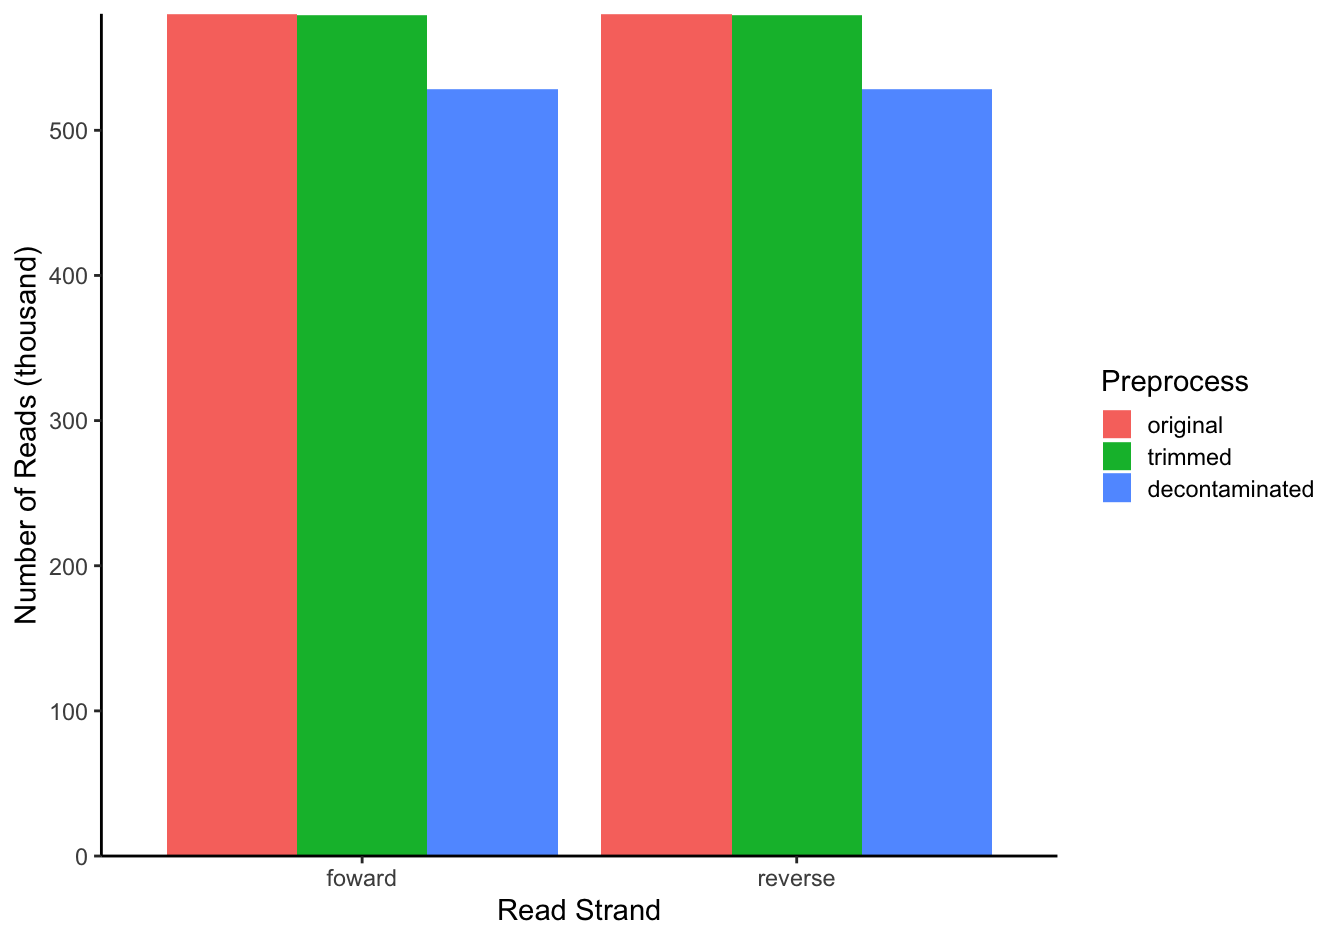
\includegraphics[width=0.8\linewidth,height=0.4\textheight]{./Figures/unnamed-chunk-2-1} \end{center}

\hypertarget{preprocess-metag-reads}{%
\chapter{Preprocessing Metagenomics Sequencing Data}\label{preprocess-metag-reads}}

\hypertarget{what-are-the-read-statistics}{%
\section{What are the read statistics}\label{what-are-the-read-statistics}}

\begin{itemize}
\tightlist
\item
  Using \texttt{seqkit\ stat} function.
\item
  Run the function on command line.
\end{itemize}

\begin{Shaded}
\begin{Highlighting}[]
\FunctionTok{mkdir} \AttributeTok{{-}p}\NormalTok{ data}
\FunctionTok{mkdir} \AttributeTok{{-}p}\NormalTok{ data/stats1  }
\ExtensionTok{seqkit}\NormalTok{ stat }\PreprocessorTok{*}\NormalTok{.fastq.gz }\OperatorTok{\textgreater{}}\NormalTok{data/stats1/seqkit\_stats.txt}
\end{Highlighting}
\end{Shaded}

\hypertarget{initial-read-quality-scores-1}{%
\section{Initial read quality scores}\label{initial-read-quality-scores-1}}

The \texttt{kneaddata} from biobakery platform is exclusively used to preprocess the metagenomics data.
- Here we set the \texttt{kneaddata} to run \texttt{fastqc} as the first step using \texttt{run-fastqc-start} function.
- Then \texttt{fastqc} results are then summarized outside \texttt{kneaddata} pipeline using \texttt{multiqc} software.

\begin{Shaded}
\begin{Highlighting}[]
\ControlFlowTok{for}\NormalTok{ i }\KeywordTok{in}\NormalTok{ data/}\PreprocessorTok{*}\NormalTok{.fastq.gz}
\ControlFlowTok{do}
\BuiltInTok{time}\NormalTok{ kneaddata }\AttributeTok{{-}{-}i} \VariableTok{$i} \DataTypeTok{\textbackslash{}}
\NormalTok{{-}o kneaddata\_fastqc1 }\DataTypeTok{\textbackslash{}}
\NormalTok{{-}{-}run{-}fastqc{-}start }\DataTypeTok{\textbackslash{}}
\NormalTok{{-}{-}bypass{-}trim }\DataTypeTok{\textbackslash{}}
\NormalTok{{-}{-}bypass{-}trf }\DataTypeTok{\textbackslash{}}
\NormalTok{{-}{-}sequencer{-}source }\StringTok{"none"} \DataTypeTok{\textbackslash{}}
\NormalTok{{-}t 4 }
\ControlFlowTok{done}


\FunctionTok{mkdir} \AttributeTok{{-}p}\NormalTok{ kneaddata\_fastqc1/multiqc1}
\ControlFlowTok{for}\NormalTok{ i }\KeywordTok{in}\NormalTok{ kneaddata\_fastqc1/fastqc}
    \ControlFlowTok{do}  
        \ExtensionTok{multiqc} \AttributeTok{{-}f} \AttributeTok{{-}{-}data{-}dir} \VariableTok{$i} \AttributeTok{{-}o}\NormalTok{ kneaddata\_fastqc1/multiqc1 }\AttributeTok{{-}{-}export}
    \ControlFlowTok{done}
\end{Highlighting}
\end{Shaded}

\hypertarget{read-trimming}{%
\section{Read Trimming}\label{read-trimming}}

\begin{itemize}
\tightlist
\item
  Using trimmomatic tool to trim the reads using the specified options.
\item
  The fastqc function is run after trimming
\item
  Then fastqc results are summarized using multiqc software.
\end{itemize}

\begin{Shaded}
\begin{Highlighting}[]

\ControlFlowTok{for}\NormalTok{ i }\KeywordTok{in}\NormalTok{ data/}\PreprocessorTok{*}\NormalTok{.fastq.gz}
\ControlFlowTok{do}
  \BuiltInTok{time}\NormalTok{ kneaddata }\AttributeTok{{-}{-}i} \VariableTok{$i} \DataTypeTok{\textbackslash{}}
    \AttributeTok{{-}o}\NormalTok{ kneaddata\_FastQC2 }\DataTypeTok{\textbackslash{}}
    \AttributeTok{{-}{-}trimmomatic}\NormalTok{ /Users/tmbuza/opt/anaconda3/envs/biobakery3/bin/ }\DataTypeTok{\textbackslash{}}
    \AttributeTok{{-}{-}trimmomatic{-}options} \DataTypeTok{\textbackslash{}}
        \StringTok{"ILLUMINACLIP:/Volumes/SeagateTMB/trimmomatic{-}0.36/adapters/NexteraPE{-}PE.fa:2:30:10 }\DataTypeTok{\textbackslash{}}
\StringTok{        LEADING:3 }\DataTypeTok{\textbackslash{}}
\StringTok{        TRAILING:3 }\DataTypeTok{\textbackslash{}}
\StringTok{        SLIDINGWINDOW:4:20 }\DataTypeTok{\textbackslash{}}
\StringTok{        MINLEN:60"} \DataTypeTok{\textbackslash{}}
    \AttributeTok{{-}{-}sequencer{-}source} \StringTok{"NexteraPE"} \DataTypeTok{\textbackslash{}}
    \AttributeTok{{-}{-}run{-}fastqc{-}end} \DataTypeTok{\textbackslash{}}
    \AttributeTok{{-}{-}bypass{-}trf} \DataTypeTok{\textbackslash{}}
    \AttributeTok{{-}t}\NormalTok{ 4 }
\ControlFlowTok{done}


\ExtensionTok{seqkit}\NormalTok{ stat kneaddata\_fastqc2/}\PreprocessorTok{*}\NormalTok{trimmed.fastq }\OperatorTok{\textgreater{}}\NormalTok{QC/QC2\_trimmed\_stats.txt}
\FunctionTok{mkdir} \AttributeTok{{-}p}\NormalTok{ kneaddata\_fastqc2/multiqc12}
\ControlFlowTok{for}\NormalTok{ i }\KeywordTok{in}\NormalTok{ kneaddata\_fastqc2/fastqc}
    \ControlFlowTok{do}  
        \ExtensionTok{multiqc} \AttributeTok{{-}f} \AttributeTok{{-}{-}data{-}dir} \VariableTok{$i} \AttributeTok{{-}o}\NormalTok{ kneaddata\_fastqc2/multiqc12 }\AttributeTok{{-}{-}export}
    \ControlFlowTok{done}
\end{Highlighting}
\end{Shaded}

\hypertarget{read-decontamination-1}{%
\section{Read Decontamination}\label{read-decontamination-1}}

\hypertarget{option-1-using-bowtie2-database}{%
\subsection{Option 1: Using Bowtie2 database}\label{option-1-using-bowtie2-database}}

\begin{itemize}
\tightlist
\item
  Trimming is done using trimmomatic
\item
  Then decontamination is done using the bowtie2 database.
\item
  Then after decontamination fastqc is implemented to assess the read quality scores of the remaining reads.
\item
  Then fastqc results are summarized using multiqc software.
\end{itemize}

\begin{Shaded}
\begin{Highlighting}[]
\ControlFlowTok{for}\NormalTok{ i }\KeywordTok{in}\NormalTok{ data/}\PreprocessorTok{*}\NormalTok{.fastq.gz}
\ControlFlowTok{do}
\BuiltInTok{time}\NormalTok{ kneaddata }\AttributeTok{{-}{-}i} \VariableTok{$i} \DataTypeTok{\textbackslash{}}
  \AttributeTok{{-}o}\NormalTok{ kneaddata\_fastqc3 }\DataTypeTok{\textbackslash{}}
      \AttributeTok{{-}{-}reference{-}db}\NormalTok{ /Volumes/SeagateTMB/kneaddata\_database/ }\DataTypeTok{\textbackslash{}}
      \AttributeTok{{-}{-}trimmomatic}\NormalTok{ /Users/tmbuza/opt/anaconda3/envs/biobakery3/bin/ }\DataTypeTok{\textbackslash{}}
      \AttributeTok{{-}{-}trimmomatic{-}options} \DataTypeTok{\textbackslash{}}
          \StringTok{"ILLUMINACLIP:/Volumes/SeagateTMB/trimmomatic{-}0.36/adapters/NexteraPE{-}PE.fa:2:30:10 }\DataTypeTok{\textbackslash{}}
\StringTok{          LEADING:3 }\DataTypeTok{\textbackslash{}}
\StringTok{          TRAILING:3 }\DataTypeTok{\textbackslash{}}
\StringTok{          SLIDINGWINDOW:4:20 }\DataTypeTok{\textbackslash{}}
\StringTok{          MINLEN:60"} \DataTypeTok{\textbackslash{}}
      \AttributeTok{{-}{-}sequencer{-}source} \StringTok{"NexteraPE"} \DataTypeTok{\textbackslash{}}
      \AttributeTok{{-}{-}run{-}trf} \DataTypeTok{\textbackslash{}}
      \AttributeTok{{-}{-}run{-}fastqc{-}end} \DataTypeTok{\textbackslash{}}
      \AttributeTok{{-}t}\NormalTok{ 4 }
\ControlFlowTok{done}

\ExtensionTok{seqkit}\NormalTok{ stat kneaddata\_fastqc3/}\PreprocessorTok{*}\NormalTok{kneaddata.fastq }\OperatorTok{\textgreater{}}\NormalTok{QC/QC3\_bowtie2decont\_stats.txt}
\FunctionTok{mkdir} \AttributeTok{{-}p}\NormalTok{ kneaddata\_fastqc3/multiqc13}
\ControlFlowTok{for}\NormalTok{ i }\KeywordTok{in}\NormalTok{ kneaddata\_fastqc3/fastqc}
    \ControlFlowTok{do}  
        \ExtensionTok{multiqc} \AttributeTok{{-}f} \AttributeTok{{-}{-}data{-}dir} \VariableTok{$i} \AttributeTok{{-}o}\NormalTok{ kneaddata\_fastqc3/multiqc13 }\AttributeTok{{-}{-}export}
    \ControlFlowTok{done}
\end{Highlighting}
\end{Shaded}

\hypertarget{option-2-using-bmtagger-database}{%
\subsection{Option 2: Using BMTagger database}\label{option-2-using-bmtagger-database}}

\begin{itemize}
\tightlist
\item
  Trimming is done using trimmomatic
\item
  Then decontamination is done using the BMTagger database.
\item
  Then after decontamination fastqc is implemented to assess the read quality scores of the remaining reads.
\item
  Then fastqc results are summarized using multiqc software.
\end{itemize}

\begin{Shaded}
\begin{Highlighting}[]
\ControlFlowTok{for}\NormalTok{ i }\KeywordTok{in}\NormalTok{ data/}\PreprocessorTok{*}\NormalTok{.fastq.gz}
\ControlFlowTok{do}
\BuiltInTok{time}\NormalTok{ kneaddata }\AttributeTok{{-}{-}i} \VariableTok{$i} \DataTypeTok{\textbackslash{}}
  \AttributeTok{{-}o}\NormalTok{ kneaddata\_fastqc4 }\DataTypeTok{\textbackslash{}}
      \AttributeTok{{-}{-}reference{-}db}\NormalTok{ /Volumes/SeagateTMB/Human\_Assembly19\_BMTagger\_DB/ }\DataTypeTok{\textbackslash{}}
      \AttributeTok{{-}{-}trimmomatic}\NormalTok{ /Users/tmbuza/opt/anaconda3/envs/biobakery3/bin/ }\DataTypeTok{\textbackslash{}}
      \AttributeTok{{-}{-}trimmomatic{-}options} \DataTypeTok{\textbackslash{}}
          \StringTok{"ILLUMINACLIP:/Volumes/SeagateTMB/trimmomatic{-}0.36/adapters/NexteraPE{-}PE.fa:2:30:10 }\DataTypeTok{\textbackslash{}}
\StringTok{          LEADING:3 }\DataTypeTok{\textbackslash{}}
\StringTok{          TRAILING:3 }\DataTypeTok{\textbackslash{}}
\StringTok{          SLIDINGWINDOW:4:20 }\DataTypeTok{\textbackslash{}}
\StringTok{          MINLEN:60"} \DataTypeTok{\textbackslash{}}
      \AttributeTok{{-}{-}sequencer{-}source} \StringTok{"NexteraPE"} \DataTypeTok{\textbackslash{}}
      \AttributeTok{{-}{-}run{-}trf} \DataTypeTok{\textbackslash{}}
      \AttributeTok{{-}{-}run{-}bmtagger} \DataTypeTok{\textbackslash{}}
      \AttributeTok{{-}{-}run{-}fastqc{-}end} \DataTypeTok{\textbackslash{}}
      \AttributeTok{{-}t}\NormalTok{ 4 }
\ControlFlowTok{done}

\ExtensionTok{seqkit}\NormalTok{ stat kneaddata\_fastqc4/}\PreprocessorTok{*}\NormalTok{kneaddata.fastq }\OperatorTok{\textgreater{}}\NormalTok{QC/QC4\_bmtaggerdecont\_stats.txt}
\FunctionTok{mkdir} \AttributeTok{{-}p}\NormalTok{ kneaddata\_fastqc4/multiqc14}
\ControlFlowTok{for}\NormalTok{ i }\KeywordTok{in}\NormalTok{ kneaddata\_fastqc4/fastqc}
    \ControlFlowTok{do}  
        \ExtensionTok{multiqc} \AttributeTok{{-}f} \AttributeTok{{-}{-}data{-}dir} \VariableTok{$i} \AttributeTok{{-}o}\NormalTok{ kneaddata\_fastqc4/multiqc14 }\AttributeTok{{-}{-}export}
    \ControlFlowTok{done}
\end{Highlighting}
\end{Shaded}

\hypertarget{taxonomic-profiling-of-microbiome-data}{%
\chapter{Taxonomic Profiling of Microbiome Data}\label{taxonomic-profiling-of-microbiome-data}}

\hypertarget{generalized-bioinformatics-workflow}{%
\section{Generalized bioinformatics workflow}\label{generalized-bioinformatics-workflow}}

\begin{center}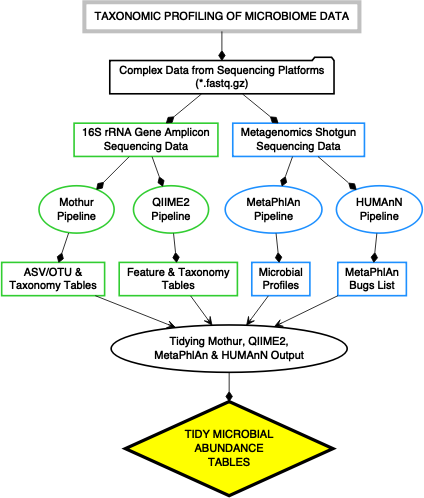
\includegraphics[width=0.8\linewidth,height=0.4\textheight]{./Figures/taxonomic_profiling_output-1} \end{center}

\hypertarget{format-of-input-data}{%
\section{Format of input data}\label{format-of-input-data}}

The default format used in this practical user guide is compressed fastq, \texttt{*.fastq.gz}.

\hypertarget{compressing-fastq-files-using-gzip}{%
\subsection{\texorpdfstring{Compressing fastq files using
\texttt{gzip}}{Compressing fastq files using gzip}}\label{compressing-fastq-files-using-gzip}}

\begin{quote}
Run the command below only if the sequencing data files are not
compressed!
\end{quote}

gzip *.fastq

\hypertarget{mcrobial-profiling-using-mothur-pipeline.}{%
\chapter{\texorpdfstring{Mcrobial profiling using \texttt{mothur} pipeline.}{Mcrobial profiling using mothur pipeline.}}\label{mcrobial-profiling-using-mothur-pipeline.}}

\hypertarget{download-a-mothur-trained-classifer}{%
\section{Download a Mothur trained classifer}\label{download-a-mothur-trained-classifer}}

\begin{itemize}
\tightlist
\item
  For demo purposes we will use \href{https://mothur.org/wiki/Silva_reference_files}{Silva seed} due to its smaller size.
\item
  Other classifiers can be found \href{https://mothur.org/wiki/taxonomy_outline/}{here}.
\end{itemize}

\begin{Shaded}
\begin{Highlighting}[]
\FunctionTok{wget}\NormalTok{ https://mothur.s3.us{-}east{-}2.amazonaws.com/wiki/silva.seed\_v138\_1.tgz}
\FunctionTok{tar}\NormalTok{ xvzf silva.seed\_v138\_1.tgz}
\FunctionTok{rm} \PreprocessorTok{*}\NormalTok{.tgz}
\end{Highlighting}
\end{Shaded}

\hypertarget{mothur-basic-wrapper}{%
\section{Mothur basic wrapper}\label{mothur-basic-wrapper}}

\begin{itemize}
\tightlist
\item
  Below is a minimal wrapper for sequence processing, classification and taxonomic assignment using \texttt{mothur} pipeline.
\item
  For more information refer to \texttt{mothur} \href{https://mothur.org/wiki/miseq_sop/}{MiSeq SOP}.
\item
  We can save this wrapper as \texttt{mothur\_code.batch} and place it in a folder named code.
\item
  Then we will run the file on command line as shown below. See the commented lines.
\item
  We assume that the input data is gunzipped i.e.~\textbf{.fastq.gz}. If not run \texttt{gzip\ *.fastq} to compress the files.
\end{itemize}

\begin{enumerate}
\def\labelenumi{\arabic{enumi}.}
\tightlist
\item
  Note that the
  \href{https://en.wikipedia.org/wiki/Shebang_(Unix)}{\texttt{shebang\ line}}
  remind us that we are running the analysis on \texttt{mothur} command
  line NOT \texttt{bash}. This takes the advantage of using the
  \textbf{current} option to refer to the last saved file.
\item
  If not generating the mapping file automatically you should make sure
  that it confer to accepted format as in
  \texttt{mothur\_mapping\_files.tsv} described in the previous section.
  In this demo we use \texttt{bush.files}. This means that all output
  files will be prefixed with the term bush to reflect the name of the
  project. Try to avoid loner names.
\end{enumerate}

\begin{Shaded}
\begin{Highlighting}[]
\CommentTok{\#!/mothur}

\CommentTok{\# Usage: mothur code/mothur\_code.batch \# if mothur is in the path}
\CommentTok{\# Usage: ./mothur code/mothur\_code.batch \# on mac/linux if the executable \textasciigrave{}mothur\textasciigrave{} is in the working directory.}
\CommentTok{\# Usage: ./mothur.exe code/mothur\_code.batch \# on Windows machins if the executable \textasciigrave{}mothur.exe\textasciigrave{} is in the working directory.}

\ExtensionTok{set.current}\ErrorTok{(}\VariableTok{processors}\OperatorTok{=}\NormalTok{1}\KeywordTok{)}
\CommentTok{\# set.logfile(name=make\_files.logfile)}
\CommentTok{\# make.file(inputdir=., type=fastq.gz, prefix=test)}

\ExtensionTok{set.logfile}\ErrorTok{(}\VariableTok{name}\OperatorTok{=}\NormalTok{seq\_assembly.logfile}\KeywordTok{)}
\ExtensionTok{make.contigs}\ErrorTok{(}\VariableTok{file}\OperatorTok{=}\NormalTok{bush.files, }\VariableTok{outputdir}\OperatorTok{=}\NormalTok{./test, }\VariableTok{maxambig}\OperatorTok{=}\NormalTok{0, }\VariableTok{maxlength}\OperatorTok{=}\NormalTok{275}\KeywordTok{);}
\ExtensionTok{unique.seqs}\ErrorTok{(}\VariableTok{count}\OperatorTok{=}\NormalTok{current}\KeywordTok{);}
\ExtensionTok{summary.seqs}\ErrorTok{(}\VariableTok{fasta}\OperatorTok{=}\NormalTok{current, }\VariableTok{count}\OperatorTok{=}\NormalTok{current}\KeywordTok{)}

\ExtensionTok{set.logfile}\ErrorTok{(}\VariableTok{name}\OperatorTok{=}\NormalTok{seq\_align\_preclustering.logfile}\KeywordTok{)}
\ExtensionTok{align.seqs}\ErrorTok{(}\VariableTok{fasta}\OperatorTok{=}\NormalTok{current, }\VariableTok{reference}\OperatorTok{=}\NormalTok{silva.seed\_v138\_1.align}\KeywordTok{);}
\ExtensionTok{screen.seqs}\ErrorTok{(}\VariableTok{fasta}\OperatorTok{=}\NormalTok{current, }\VariableTok{count}\OperatorTok{=}\NormalTok{current, }\VariableTok{start}\OperatorTok{=}\NormalTok{13862, }\VariableTok{end}\OperatorTok{=}\NormalTok{23444, }\VariableTok{maxhomop}\OperatorTok{=}\NormalTok{8}\KeywordTok{);}
\ExtensionTok{filter.seqs}\ErrorTok{(}\VariableTok{fasta}\OperatorTok{=}\NormalTok{current, }\VariableTok{vertical}\OperatorTok{=}\NormalTok{T, }\VariableTok{trump}\OperatorTok{=}\NormalTok{.}\KeywordTok{);}
\ExtensionTok{pre.cluster}\ErrorTok{(}\VariableTok{fasta}\OperatorTok{=}\NormalTok{current, }\VariableTok{count}\OperatorTok{=}\NormalTok{current, }\VariableTok{diffs}\OperatorTok{=}\NormalTok{2}\KeywordTok{);}
\ExtensionTok{unique.seqs}\ErrorTok{(}\VariableTok{fasta}\OperatorTok{=}\NormalTok{current, }\VariableTok{count}\OperatorTok{=}\NormalTok{current}\KeywordTok{);}

\ExtensionTok{set.logfile}\ErrorTok{(}\VariableTok{name}\OperatorTok{=}\NormalTok{chimera\_removal.logfile}\KeywordTok{)}
\ExtensionTok{chimera.vsearch}\ErrorTok{(}\VariableTok{fasta}\OperatorTok{=}\NormalTok{current, }\VariableTok{count}\OperatorTok{=}\NormalTok{current, }\VariableTok{dereplicate}\OperatorTok{=}\NormalTok{t}\KeywordTok{);}

\ExtensionTok{set.logfile}\ErrorTok{(}\VariableTok{name}\OperatorTok{=}\NormalTok{silva\_seed\_classification.logfile}\KeywordTok{)}
\ExtensionTok{classify.seqs}\ErrorTok{(}\VariableTok{fasta}\OperatorTok{=}\NormalTok{current, }\VariableTok{count}\OperatorTok{=}\NormalTok{current, }\VariableTok{reference}\OperatorTok{=}\NormalTok{silva.seed\_v138\_1.align, }\VariableTok{taxonomy}\OperatorTok{=}\NormalTok{silva.seed\_v138\_1.tax, }\VariableTok{cutoff}\OperatorTok{=}\NormalTok{100}\KeywordTok{);}
\ExtensionTok{remove.lineage}\ErrorTok{(}\VariableTok{fasta}\OperatorTok{=}\NormalTok{current, }\VariableTok{count}\OperatorTok{=}\NormalTok{current, }\VariableTok{taxonomy}\OperatorTok{=}\NormalTok{current, }\VariableTok{taxon}\OperatorTok{=}\NormalTok{Chloroplast{-}Mitochondria{-}unknown{-}Archaea{-}Eukaryota}\KeywordTok{);}

\ExtensionTok{set.logfile}\ErrorTok{(}\VariableTok{name}\OperatorTok{=}\NormalTok{final\_files.logfile}\KeywordTok{)}
\ExtensionTok{rename.file}\ErrorTok{(}\VariableTok{fasta}\OperatorTok{=}\NormalTok{current, }\VariableTok{count}\OperatorTok{=}\NormalTok{current, }\VariableTok{taxonomy}\OperatorTok{=}\NormalTok{current, }\VariableTok{prefix}\OperatorTok{=}\NormalTok{final}\KeywordTok{)}

\ExtensionTok{set.logfile}\ErrorTok{(}\VariableTok{name}\OperatorTok{=}\NormalTok{otu\_clustering.logfile}\KeywordTok{)}
\ExtensionTok{dist.seqs}\ErrorTok{(}\VariableTok{fasta}\OperatorTok{=}\NormalTok{current, }\VariableTok{cutoff}\OperatorTok{=}\NormalTok{0.03}\KeywordTok{);}
\ExtensionTok{cluster}\ErrorTok{(}\VariableTok{column}\OperatorTok{=}\NormalTok{current, }\VariableTok{count}\OperatorTok{=}\NormalTok{current, }\VariableTok{cutoff}\OperatorTok{=}\NormalTok{0.03}\KeywordTok{);}
\ExtensionTok{make.shared}\ErrorTok{(}\VariableTok{list}\OperatorTok{=}\NormalTok{current, }\VariableTok{count}\OperatorTok{=}\NormalTok{current, }\VariableTok{label}\OperatorTok{=}\NormalTok{0.03}\KeywordTok{);}
\ExtensionTok{classify.otu}\ErrorTok{(}\VariableTok{list}\OperatorTok{=}\NormalTok{current, }\VariableTok{count}\OperatorTok{=}\NormalTok{current, }\VariableTok{taxonomy}\OperatorTok{=}\NormalTok{current, }\VariableTok{label}\OperatorTok{=}\NormalTok{0.03}\KeywordTok{);}
\ExtensionTok{make.lefse}\ErrorTok{(}\VariableTok{shared}\OperatorTok{=}\NormalTok{current, }\VariableTok{constaxonomy}\OperatorTok{=}\NormalTok{current}\KeywordTok{);}
\ExtensionTok{make.biom}\ErrorTok{(}\VariableTok{shared}\OperatorTok{=}\NormalTok{current, }\VariableTok{constaxonomy}\OperatorTok{=}\NormalTok{current}\KeywordTok{);}

\ExtensionTok{set.logfile}\ErrorTok{(}\VariableTok{name}\OperatorTok{=}\NormalTok{phylotype\_clustering.logfile}\KeywordTok{)}
\ExtensionTok{phylotype}\ErrorTok{(}\VariableTok{taxonomy}\OperatorTok{=}\NormalTok{current}\KeywordTok{);}
\ExtensionTok{make.shared}\ErrorTok{(}\VariableTok{list}\OperatorTok{=}\NormalTok{current, }\VariableTok{count}\OperatorTok{=}\NormalTok{current, }\VariableTok{label}\OperatorTok{=}\NormalTok{1}\KeywordTok{);}
\ExtensionTok{classify.otu}\ErrorTok{(}\VariableTok{list}\OperatorTok{=}\NormalTok{current, }\VariableTok{count}\OperatorTok{=}\NormalTok{current, }\VariableTok{taxonomy}\OperatorTok{=}\NormalTok{current, }\VariableTok{label}\OperatorTok{=}\NormalTok{1}\KeywordTok{);}
\ExtensionTok{make.lefse}\ErrorTok{(}\VariableTok{shared}\OperatorTok{=}\NormalTok{current, }\VariableTok{constaxonomy}\OperatorTok{=}\NormalTok{current}\KeywordTok{);}
\ExtensionTok{make.biom}\ErrorTok{(}\VariableTok{shared}\OperatorTok{=}\NormalTok{current, }\VariableTok{constaxonomy}\OperatorTok{=}\NormalTok{current}\KeywordTok{);}

\ExtensionTok{set.logfile}\ErrorTok{(}\VariableTok{name}\OperatorTok{=}\NormalTok{asv\_clustering.logfile}\KeywordTok{)}
\ExtensionTok{make.shared}\ErrorTok{(}\VariableTok{count}\OperatorTok{=}\NormalTok{current}\KeywordTok{)}
\ExtensionTok{classify.otu}\ErrorTok{(}\VariableTok{list}\OperatorTok{=}\NormalTok{current, }\VariableTok{count}\OperatorTok{=}\NormalTok{current, }\VariableTok{taxonomy}\OperatorTok{=}\NormalTok{current, }\VariableTok{label}\OperatorTok{=}\NormalTok{ASV}\KeywordTok{)}
\ExtensionTok{make.lefse}\ErrorTok{(}\VariableTok{shared}\OperatorTok{=}\NormalTok{current, }\VariableTok{constaxonomy}\OperatorTok{=}\NormalTok{current}\KeywordTok{)}
\ExtensionTok{make.biom}\ErrorTok{(}\VariableTok{shared}\OperatorTok{=}\NormalTok{current, }\VariableTok{constaxonomy}\OperatorTok{=}\NormalTok{current}\KeywordTok{)}

\ExtensionTok{set.logfile}\ErrorTok{(}\VariableTok{name}\OperatorTok{=}\NormalTok{phylogenetic\_clustering.logfile}\KeywordTok{)}
\ExtensionTok{dist.seqs}\ErrorTok{(}\VariableTok{fasta}\OperatorTok{=}\NormalTok{current, }\VariableTok{output}\OperatorTok{=}\NormalTok{lt}\KeywordTok{)}
\ExtensionTok{clearcut}\ErrorTok{(}\VariableTok{phylip}\OperatorTok{=}\NormalTok{current}\KeywordTok{)}
\end{Highlighting}
\end{Shaded}

\hypertarget{mcrobial-profiling-using-qiime2-pipeline}{%
\chapter{\texorpdfstring{Mcrobial profiling using \texttt{qiime2} pipeline}{Mcrobial profiling using qiime2 pipeline}}\label{mcrobial-profiling-using-qiime2-pipeline}}

\hypertarget{download-a-qiime2-trained-classifer}{%
\subsection{Download a QIIME2 trained classifer}\label{download-a-qiime2-trained-classifer}}

\begin{itemize}
\tightlist
\item
  You can use Naive Bayes (nb) classifiers trained on GreenGenes or SILVA database with 99\% OTUs. You can train your own classifier using the \href{https://github.com/qiime2/q2-feature-classifier}{q2-feature-classifier}.
\end{itemize}

Here we will download the smallest classifier, the naive classifier trained on \href{https://docs.qiime2.org/2022.2/data-resources/}{Greengenes 13\_8 99\% OTUs from 515F/806R region of sequences}

\begin{Shaded}
\begin{Highlighting}[]
\FunctionTok{wget} \DataTypeTok{\textbackslash{}}
  \AttributeTok{{-}O} \StringTok{"gg{-}13{-}8{-}99{-}515{-}806{-}nb{-}classifier.qza"} \DataTypeTok{\textbackslash{}}
  \StringTok{"https://data.qiime2.org/2022.2/common/gg{-}13{-}8{-}99{-}515{-}806{-}nb{-}classifier.qza"}
\end{Highlighting}
\end{Shaded}

\hypertarget{qiime2-installation}{%
\subsection{QIIME2 installation}\label{qiime2-installation}}

\begin{itemize}
\tightlist
\item
  We assumes that you have already installed QIIME 2. If not please do so using the instructions described \href{https://docs.qiime2.org/2022.2/install/}{here!}.
\end{itemize}

A simple demo for installing qiime2 on Mac OS

\begin{Shaded}
\begin{Highlighting}[]
\FunctionTok{wget}\NormalTok{ https://data.qiime2.org/distro/core/qiime2{-}2022.2{-}py38{-}osx{-}conda.yml}
\ExtensionTok{conda}\NormalTok{ env create }\AttributeTok{{-}n}\NormalTok{ qiime2{-}2022.2 }\AttributeTok{{-}{-}file}\NormalTok{ qiime2{-}2022.2{-}py38{-}osx{-}conda.yml}
\FunctionTok{rm}\NormalTok{ qiime2{-}2022.2{-}py39{-}osx{-}conda.yml}

\CommentTok{\# Activate qiime environment }
\ExtensionTok{conda}\NormalTok{ activate qiime2{-}2022.2}

\CommentTok{\# Confirm installation}
\ExtensionTok{qiime}\NormalTok{ info}
\end{Highlighting}
\end{Shaded}

\hypertarget{running-qiime2-commands}{%
\subsection{Running QIIME2 commands}\label{running-qiime2-commands}}

\begin{itemize}
\tightlist
\item
  We prefer to use the command line interface \href{https://docs.qiime2.org/2022.2/interfaces/q2cli/}{g2cli}.
\item
  Activate the qiime2 environment: We are using qiime2-2022.2.
\end{itemize}

\begin{Shaded}
\begin{Highlighting}[]
\ExtensionTok{conda}\NormalTok{ activate qiime2{-}2022.2}
\end{Highlighting}
\end{Shaded}

\hypertarget{import-paired-end-fastq-files}{%
\subsection{Import paired-end fastq files}\label{import-paired-end-fastq-files}}

\begin{Shaded}
\begin{Highlighting}[]
\ExtensionTok{qiime}\NormalTok{ tools import }\DataTypeTok{\textbackslash{}}
  \AttributeTok{{-}{-}type} \StringTok{\textquotesingle{}SampleData[PairedEndSequencesWithQuality]\textquotesingle{}} \DataTypeTok{\textbackslash{}}
  \AttributeTok{{-}{-}input{-}path}\NormalTok{ pe{-}33{-}manifest.tsv }\DataTypeTok{\textbackslash{}}
  \AttributeTok{{-}{-}output{-}path}\NormalTok{ qiime2\_bushmeat/paired{-}end{-}demux.qza }\DataTypeTok{\textbackslash{}}
  \AttributeTok{{-}{-}input{-}format}\NormalTok{ PairedEndFastqManifestPhred33V2}
\end{Highlighting}
\end{Shaded}

\begin{itemize}
\tightlist
\item
  Below is a minimal wrapper for

  \begin{itemize}
  \tightlist
  \item
    exploring the metadata,
  \item
    importing the data,
  \item
    sequence quality control,
  \item
    sequence classification,
  \item
    taxonomic assignment,
  \item
    generating feature table.
  \end{itemize}
\end{itemize}

For more information refer to \texttt{qiime2} \href{https://docs.qiime2.org/2022.2/tutorials/}{tutorials}.

\begin{Shaded}
\begin{Highlighting}[]
\CommentTok{\#!/qiime}

\CommentTok{\# Usage: qiime2 code/qiime2\_code.bash}
\end{Highlighting}
\end{Shaded}

\hypertarget{qiime2-output-tidying}{%
\section{QIIME2 output tidying}\label{qiime2-output-tidying}}

\begin{Shaded}
\begin{Highlighting}[]
\NormalTok{taxlevels }\OtherTok{\textless{}{-}} \FunctionTok{c}\NormalTok{(}\StringTok{"kingdom"}\NormalTok{, }\StringTok{"phylum"}\NormalTok{, }\StringTok{"class"}\NormalTok{, }\StringTok{"order"}\NormalTok{, }\StringTok{"family"}\NormalTok{, }\StringTok{"genus"}\NormalTok{, }\StringTok{"species"}\NormalTok{)}

\FunctionTok{read\_delim}\NormalTok{(}\StringTok{"/Volumes/RedSeagate/MOTHUR\_BUSHMEAT/SRR7450/qiime2\_bushmeat/q2{-}transformed{-}tables/taxonomy.tsv"}\NormalTok{) }\SpecialCharTok{\%\textgreater{}\%}
  \FunctionTok{rename\_all}\NormalTok{(tolower) }\SpecialCharTok{\%\textgreater{}\%}
  \FunctionTok{rename}\NormalTok{(}\AttributeTok{otu =} \StringTok{"feature id"}\NormalTok{) }\SpecialCharTok{\%\textgreater{}\%} 
  \FunctionTok{mutate}\NormalTok{(}\AttributeTok{confidence =} \FunctionTok{round}\NormalTok{(confidence, }\AttributeTok{digits =} \DecValTok{2}\NormalTok{)) }\SpecialCharTok{\%\textgreater{}\%}
  \CommentTok{\# filter(confidence == 1.00) \%\textgreater{}\% }
  \FunctionTok{mutate}\NormalTok{(}\AttributeTok{taxon =} \FunctionTok{str\_replace\_all}\NormalTok{(taxon, }\StringTok{"; s\_\_$"}\NormalTok{, }\StringTok{""}\NormalTok{),}
         \AttributeTok{taxon =} \FunctionTok{str\_replace\_all}\NormalTok{(taxon, }\StringTok{"; g\_\_$"}\NormalTok{, }\StringTok{""}\NormalTok{),}
         \AttributeTok{taxon =} \FunctionTok{str\_replace\_all}\NormalTok{(taxon, }\StringTok{"; f\_\_$"}\NormalTok{, }\StringTok{""}\NormalTok{),}
         \AttributeTok{taxon =} \FunctionTok{str\_replace\_all}\NormalTok{(taxon, }\StringTok{"; o\_\_$"}\NormalTok{, }\StringTok{""}\NormalTok{),}
         \AttributeTok{taxon =} \FunctionTok{str\_replace\_all}\NormalTok{(taxon, }\StringTok{"; c\_\_$"}\NormalTok{, }\StringTok{""}\NormalTok{),}
         \AttributeTok{taxon =} \FunctionTok{str\_replace\_all}\NormalTok{(taxon, }\StringTok{"; p\_\_$"}\NormalTok{, }\StringTok{""}\NormalTok{),}
         \AttributeTok{taxon =} \FunctionTok{str\_replace\_all}\NormalTok{(taxon, }\StringTok{"; k\_\_$"}\NormalTok{, }\StringTok{""}\NormalTok{),}
\NormalTok{         ) }\SpecialCharTok{\%\textgreater{}\%} 
  \FunctionTok{separate}\NormalTok{(}\AttributeTok{col =}\NormalTok{ taxon, }\AttributeTok{into =} \FunctionTok{all\_of}\NormalTok{(taxlevels), }\AttributeTok{sep =} \StringTok{"; "}\NormalTok{) }\SpecialCharTok{\%\textgreater{}\%}
  \FunctionTok{saveRDS}\NormalTok{(}\StringTok{"RDataRDS/q2\_taxonomy.rds"}\NormalTok{)}
\end{Highlighting}
\end{Shaded}

\begin{Shaded}
\begin{Highlighting}[]
\FunctionTok{read\_delim}\NormalTok{(}\StringTok{"/Volumes/RedSeagate/MOTHUR\_BUSHMEAT/SRR7450/qiime2\_bushmeat/q2{-}transformed{-}tables/feature{-}table.tsv"}\NormalTok{, }\AttributeTok{skip =} \DecValTok{1}\NormalTok{) }\SpecialCharTok{\%\textgreater{}\%}
  \FunctionTok{rename}\NormalTok{(}\AttributeTok{otu =} \StringTok{"\#OTU ID"}\NormalTok{) }\SpecialCharTok{\%\textgreater{}\%} 
  \FunctionTok{saveRDS}\NormalTok{(}\StringTok{"RDataRDS/q2\_otutable.rds"}\NormalTok{)}
\end{Highlighting}
\end{Shaded}

\begin{Shaded}
\begin{Highlighting}[]
\FunctionTok{readRDS}\NormalTok{(}\StringTok{"RDataRDS/q2\_taxonomy.rds"}\NormalTok{) }\SpecialCharTok{\%\textgreater{}\%} 
  \FunctionTok{inner\_join}\NormalTok{(., }\FunctionTok{readRDS}\NormalTok{(}\StringTok{"RDataRDS/q2\_otutable.rds"}\NormalTok{), }\AttributeTok{by=}\StringTok{"otu"}\NormalTok{)}
\end{Highlighting}
\end{Shaded}

\begin{verbatim}
# A tibble: 494 x 19
   otu     kingdom phylum class order family genus species confidence SRR7450728
   <chr>   <chr>   <chr>  <chr> <chr> <chr>  <chr> <chr>        <dbl>      <dbl>
 1 04edaa~ k__Bac~ p__Fi~ c__C~ o__C~ f__Pe~ g__[~ s__sor~       0.96        267
 2 e27b9e~ k__Bac~ p__Fi~ c__B~ o__B~ f__St~ g__M~ s__cas~       0.91      15210
 3 d46e22~ k__Bac~ p__Pr~ c__G~ o__E~ f__En~ <NA>  <NA>          1          2374
 4 41db43~ k__Bac~ <NA>   <NA>  <NA>  <NA>   <NA>  <NA>          0.93        409
 5 9580aa~ k__Bac~ p__Fi~ c__C~ o__C~ f__Cl~ g__C~ s__per~       1           146
 6 6f70e5~ k__Bac~ p__Fi~ c__C~ o__C~ f__Cl~ g__C~ <NA>          0.8           0
 7 547357~ k__Bac~ <NA>   <NA>  <NA>  <NA>   <NA>  <NA>          0.97       7092
 8 bc3621~ k__Bac~ p__Pr~ c__G~ o__P~ f__Mo~ g__A~ <NA>          1           357
 9 9209e4~ k__Bac~ p__Fi~ c__C~ o__C~ f__Cl~ g__C~ <NA>          0.98        689
10 5970d8~ k__Bac~ p__Cy~ c__C~ o__C~ <NA>   <NA>  <NA>          1           111
# ... with 484 more rows, and 9 more variables: SRR7450732 <dbl>,
#   SRR7450746 <dbl>, SRR7450747 <dbl>, SRR7450752 <dbl>, SRR7450753 <dbl>,
#   SRR7450755 <dbl>, SRR7450757 <dbl>, SRR7450758 <dbl>, SRR7450759 <dbl>
\end{verbatim}

\hypertarget{taxonomic-profiling-of-metagenomics-sequencing-data}{%
\chapter{Taxonomic Profiling of Metagenomics Sequencing Data}\label{taxonomic-profiling-of-metagenomics-sequencing-data}}

\hypertarget{using-metaphlan-pipeline.}{%
\section{Using MetaPhlAn pipeline.}\label{using-metaphlan-pipeline.}}

\begin{itemize}
\tightlist
\item
  We loop through the fastq files using the following parameters.
\item
  You can optionally customize these parameters to suit your needs.
\item
  Note that most parameters are default setting except the \emph{-t rel\_ab\_w\_read\_stats} which will add the read count to the output.
\end{itemize}

\begin{Shaded}
\begin{Highlighting}[]

\ControlFlowTok{for}\NormalTok{ i }\KeywordTok{in}\NormalTok{ data/}\PreprocessorTok{*}\NormalTok{.fastq.gz}
    \ControlFlowTok{do} 
        \ExtensionTok{metaphlan} \VariableTok{$i} \DataTypeTok{\textbackslash{}}
        \AttributeTok{{-}{-}input\_type}\NormalTok{ fastq }\DataTypeTok{\textbackslash{}}
        \AttributeTok{{-}{-}force} \DataTypeTok{\textbackslash{}}
        \AttributeTok{{-}{-}bowtie2db}\NormalTok{ /Volumes/SeagateTMB/metaphlan\_databases/ }\DataTypeTok{\textbackslash{}}
        \AttributeTok{{-}{-}nproc}\NormalTok{ 4 }\DataTypeTok{\textbackslash{}}
        \AttributeTok{{-}{-}stat\_q}\NormalTok{ 0.02 }\DataTypeTok{\textbackslash{}}
        \AttributeTok{{-}{-}min\_mapq\_val}\NormalTok{ 5 }\DataTypeTok{\textbackslash{}}
        \AttributeTok{{-}{-}output\_file} \VariableTok{$\{i}\OperatorTok{\%}\VariableTok{\}}\NormalTok{\_metaphlan3\_profile.txt }\DataTypeTok{\textbackslash{}}
        \AttributeTok{{-}{-}bowtie2out} \VariableTok{$\{i}\OperatorTok{\%}\VariableTok{\}}\NormalTok{\_metaphlan3\_bowtie2out.txt }\DataTypeTok{\textbackslash{}}
        \AttributeTok{{-}{-}biom} \VariableTok{$\{i}\OperatorTok{\%}\VariableTok{\}}\NormalTok{\_metaphlan3\_abundance.biom }\DataTypeTok{\textbackslash{}}
    \AttributeTok{{-}t}\NormalTok{ rel\_ab\_w\_read\_stats}
    \ControlFlowTok{done}
\end{Highlighting}
\end{Shaded}

\hypertarget{output-of-taxonomic-profiling}{%
\section{Output of taxonomic profiling}\label{output-of-taxonomic-profiling}}

\begin{itemize}
\tightlist
\item
  OTU table in mothur and QIIME2
\item
  MetaPhlAn pipeline output taxonomic profiles for each input fastq file.
\item
  You can further use some integrated functions to manage the output. For example, the command below merge relative abundance into a single file similar to a transposed OTU table from Mothur and QIIME platforms.
\end{itemize}

\hypertarget{appendix-appendix}{%
\appendix}


\hypertarget{saved-data-objects}{%
\chapter{Saved Data Objects}\label{saved-data-objects}}

\hypertarget{rds-format-for-individual-object}{%
\section{RDS Format for Individual Object}\label{rds-format-for-individual-object}}

\begin{verbatim}
[1] "./RDataRDS/metadata.rds"     "./RDataRDS/q2_otutable.rds" 
[3] "./RDataRDS/q2_taxonomy.rds"  "./RDataRDS/seqkit_stats.rds"
\end{verbatim}

\hypertarget{rdata-format-for-multiple-objects}{%
\section{RData Format for Multiple Objects}\label{rdata-format-for-multiple-objects}}

\begin{verbatim}
[1] "./RDataRDS/saved_objects.RData"
\end{verbatim}

\hypertarget{csv-format-for-selected-dataframe}{%
\section{CSV Format for Selected Dataframe}\label{csv-format-for-selected-dataframe}}

\begin{verbatim}
character(0)
\end{verbatim}

\hypertarget{how-to-reload-rds-or-rdata-into-r-environment}{%
\section{How to reload RDS or RData into R environment}\label{how-to-reload-rds-or-rdata-into-r-environment}}

\begin{tmbarrowF}
\begin{itemize}
\tightlist
\item
  RDS format e.g.~foo.rds

  \begin{itemize}
  \tightlist
  \item
    foo \textless- readRDS(``RDataRDS/foo.rds'')
  \end{itemize}
\item
  RData format e.g.~foo.RData

  \begin{itemize}
  \tightlist
  \item
    load(``RDataRDS/foo.RData'', verbose = TRUE)
  \end{itemize}
\item
  List objects in RData

  \begin{itemize}
  \tightlist
  \item
    lsdata(``foo.RData'')
  \end{itemize}
\end{itemize}
\end{tmbarrowF}

\hypertarget{software-and-packages-used}{%
\chapter{Software and Packages Used}\label{software-and-packages-used}}

\hypertarget{basic-dependencies}{%
\section{Basic dependencies}\label{basic-dependencies}}

\begin{itemize}
\tightlist
\item
  R version 4.1.3 (2022-03-10)
\item
  \texttt{tidyverse} (v. 1.3.1)
\item
  \texttt{bookdown} (v. 0.25)
\item
  \texttt{ggpubr} (v. 0.4.0)
\item
  \texttt{downlit} (v. 0.4.0)
\item
  \texttt{phyloseq} (v. 1.38.0)
\item
  \texttt{ape} (v. 5.6.2)
\item
  \texttt{ggtext} (v. 0.1.1)
\item
  \texttt{dendextend} (v. 1.15.2)
\item
  \texttt{metagMisc} (v. 0.0.4)
\item
  \texttt{cgwtools} (v. 3.3)
\end{itemize}

\hypertarget{available-on-machine-used}{%
\section{Available on machine used}\label{available-on-machine-used}}

\begin{verbatim}
R version 4.1.3 (2022-03-10)
Platform: x86_64-apple-darwin17.0 (64-bit)
Running under: macOS Big Sur/Monterey 10.16

Matrix products: default
BLAS:   /Library/Frameworks/R.framework/Versions/4.1/Resources/lib/libRblas.0.dylib
LAPACK: /Library/Frameworks/R.framework/Versions/4.1/Resources/lib/libRlapack.dylib

locale:
[1] en_US.UTF-8/en_US.UTF-8/en_US.UTF-8/C/en_US.UTF-8/en_US.UTF-8

attached base packages:
[1] stats     graphics  grDevices utils     datasets  methods   base     

other attached packages:
 [1] DiagrammeRsvg_0.1 DiagrammeR_1.0.9  cgwtools_3.3      metagMisc_0.0.4  
 [5] dendextend_1.15.2 ggtext_0.1.1      ape_5.6-2         phyloseq_1.38.0  
 [9] downlit_0.4.0     ggpubr_0.4.0      bookdown_0.25     rmarkdown_2.13   
[13] knitr_1.38        forcats_0.5.1     stringr_1.4.0     dplyr_1.0.8      
[17] purrr_0.3.4       readr_2.1.2       tidyr_1.2.0       tibble_3.1.6     
[21] ggplot2_3.3.5     tidyverse_1.3.1  

loaded via a namespace (and not attached):
  [1] readxl_1.4.0           backports_1.4.1        plyr_1.8.7            
  [4] igraph_1.2.11          splines_4.1.3          gmp_0.6-5             
  [7] GenomeInfoDb_1.30.1    digest_0.6.29          foreach_1.5.2         
 [10] htmltools_0.5.2        viridis_0.6.2          magick_2.7.3          
 [13] fansi_1.0.3            magrittr_2.0.3         memoise_2.0.1         
 [16] cluster_2.1.2          tzdb_0.3.0             Biostrings_2.62.0     
 [19] modelr_0.1.8           vroom_1.5.7            colorspace_2.0-3      
 [22] rvest_1.0.2            haven_2.4.3            xfun_0.30             
 [25] callr_3.7.0            crayon_1.5.1           RCurl_1.98-1.6        
 [28] jsonlite_1.8.0         survival_3.3-1         iterators_1.0.14      
 [31] glue_1.6.2             gtable_0.3.0           zlibbioc_1.40.0       
 [34] XVector_0.34.0         webshot_0.5.3          V8_4.1.0              
 [37] car_3.0-12             Rhdf5lib_1.16.0        BiocGenerics_0.40.0   
 [40] abind_1.4-5            scales_1.1.1           DBI_1.1.2             
 [43] rstatix_0.7.0          Rcpp_1.0.8.3           viridisLite_0.4.0     
 [46] gridtext_0.1.4         bit_4.0.4              stats4_4.1.3          
 [49] htmlwidgets_1.5.4      httr_1.4.2             RColorBrewer_1.1-2    
 [52] ellipsis_0.3.2         pkgconfig_2.0.3        farver_2.1.0          
 [55] dbplyr_2.1.1           utf8_1.2.2             tidyselect_1.1.2      
 [58] labeling_0.4.2         rlang_1.0.2            reshape2_1.4.4        
 [61] munsell_0.5.0          cellranger_1.1.0       tools_4.1.3           
 [64] visNetwork_2.1.0       cachem_1.0.6           cli_3.2.0             
 [67] generics_0.1.2         ade4_1.7-18            broom_0.7.12          
 [70] evaluate_0.15          biomformat_1.22.0      fastmap_1.1.0         
 [73] yaml_2.3.5             processx_3.5.3         bit64_4.0.5           
 [76] fs_1.5.2               nlme_3.1-157           xml2_1.3.3            
 [79] compiler_4.1.3         rstudioapi_0.13        curl_4.3.2            
 [82] ggsignif_0.6.3         reprex_2.0.1           stringi_1.7.6         
 [85] ps_1.6.0               lattice_0.20-45        Matrix_1.4-1          
 [88] markdown_1.1           vegan_2.5-7            permute_0.9-7         
 [91] multtest_2.50.0        vctrs_0.4.0            pillar_1.7.0          
 [94] lifecycle_1.0.1        rhdf5filters_1.6.0     data.table_1.14.2     
 [97] bitops_1.0-7           R6_2.5.1               gridExtra_2.3         
[100] IRanges_2.28.0         codetools_0.2-18       MASS_7.3-56           
[103] assertthat_0.2.1       rhdf5_2.38.1           withr_2.5.0           
[106] S4Vectors_0.32.3       GenomeInfoDbData_1.2.7 mgcv_1.8-39           
[109] parallel_4.1.3         hms_1.1.1              grid_4.1.3            
[112] carData_3.0-5          Biobase_2.54.0         lubridate_1.8.0       
\end{verbatim}

  \bibliography{library/book.bib,library/packages.bib,library/microbiome.bib,library/software.bib}

\end{document}
